\chapter{Results and Discussion}

\section{Project Outcomes}

The project produced a working end-to-end system, which is summarised below.

\begin{itemize}
\item \textbf{Rover and firmware.} Two sketches (Nano and ESP32-CAM) that compile without warnings, a documented HTTP API and UART
      protocol, per-sensor power switches with heater warm-up handling, and bring-up tools that check the wiring and the API.
\item \textbf{Backend.} A validated, timestamped ingestion path; deterministic window, daily and on/off-log chunks; a knowledge store with hybrid
      retrieval; Pipeline A (planner, exact facts, citation-validated answers, streaming); Pipeline B (vision call, bounded research agent,
      one-way write); a live activity stream; a browser interface; a rover simulator; and demonstration data with a loader.
\item \textbf{Mobile application.} Six screens (overview, rover control with sensor switches, diagnosis, streamed chat, sensors, Live view)
      built into an installable Android package by a GitHub Actions workflow.
\item \textbf{Quality evidence.} 96 backend and 22 application automated tests, provider contract tests against local fake services, a ten-question
      evaluation with ground truth computed from raw data, and measured performance figures.
\item \textbf{Responsible-AI features.} Uncalibrated-confidence disclosure, possibility-phrased diagnoses, evidence separated from assumptions,
      removal of invented citations, explicit gap reporting, deletion of images and chunks, and chemical-safety rules.
\end{itemize}

\section{Result Analysis}

\subsection{Pipeline A Evaluation}

Table~\ref{tab:evalresults} reports the ten-question evaluation (Section~6.2) in two configurations that need no cloud key: the offline
mode (rule-based planner, extractive answers, hashing embedder) and a local language model (Gemma served by Ollama, hashing
embedder). The raw reports are stored with the project (\texttt{docs/evaluation-offline.json} and
\texttt{docs/evaluation-local-llm.json}).

\begin{table}[H]
\centering
\caption{Pipeline A evaluation on the synthetic farm (10 questions).}
\label{tab:evalresults}
\small
\begin{tabular}{|P{5.4cm}|c|c|c|}
\hline
\textbf{Measure} & \textbf{Offline} & \textbf{Local LLM, first run} & \textbf{Local LLM, final}\\\hline
Planner accuracy & 100\,\% & 90\,\% & 100\,\%\\\hline
Numeric recall & 100\,\% & 83\,\% & 100\,\%\\\hline
Citation accuracy (expected evidence type) & 100\,\% & 80\,\% & 100\,\%\\\hline
Keyword accuracy & 100\,\% & 100\,\% & 100\,\%\\\hline
Answers carrying citations & 100\,\% & -- & 100\,\%\\\hline
Median latency per answer & 11.5\,ms & 13.5\,s & 18.9\,s\\\hline
\end{tabular}
\end{table}

\noindent\textbf{Interpretation.} The offline result shows that the deterministic part of the system, which computes the facts and
retrieves the chunks, is correct on all ten questions. The first local-model run shows the value of the evaluation: it exposed
four failures that were traced to missing excursion facts and a planner that mislabelled past periods, and the fixes made the
system more robust for every model. These are single runs on a benchmark of ten questions, so they demonstrate correct behaviour on representative
questions; they are not a general accuracy claim. A larger question set and a run with the cloud model are the natural next steps.
\placeholderblock{Add a third column here after running the RAG evaluation script with your Gemini key (see the project README).}

\subsection{Sensor Gaps}

The sensor-switch feature was verified by tests that build a day with the gas sensors on, then off, then the rover disconnected, and then
a stretch of video-only mode. The tests check the recorded events, the status of each five-minute bucket, the text of the window,
daily and on/off-log chunks, the facts, and the prompt that reaches the model. In a live run with the rover simulator, switching MQ5
and MQ6 off through the backend relay reached the rover, the rover's next push updated the backend within seconds, readings stopped, and the Live
view showed each switch as an event.

\section{Generated Output Analysis}

\subsection{A Window Chunk}

The text that is embedded for a 15-minute window is deterministic. This is a real chunk from the demonstration data
(Section~5.2 shows the format): it contains the numbers with the interpretation band of each average, and nothing that was invented.

\subsection{An Answer about a Switched-off Sensor}

The following facts are the real output of the backend (offline mode, so the facts are listed directly) for the question
``What were the gas readings this morning?'' in the demonstration data, where the gas sensors had been switched off:

\begin{lstlisting}
- No mq5 gas index (lpg / natural gas / methane) readings were recorded this
  morning (Sat 17 Oct 2026, 05:00-12:00). [F1]
- No mq6 gas index (lpg / butane / propane) readings were recorded this
  morning (Sat 17 Oct 2026, 05:00-12:00). [F2]
- Sensor on/off history this morning (Sat 17 Oct 2026, 05:00-12:00) (farm time):
  MQ5: switched off 06:00-09:20; rover not connected for 3 h 40 min of the
  period. MQ6: switched off 06:00-09:20; rover not connected for 3 h 40 min
  of the period. [F3]
\end{lstlisting}

\noindent With a language model configured, these facts form the context of the answer, and the prompt makes the model state the periods and
the tip to switch the sensors on, without estimating any value.

\subsection{A Diagnosis with a Local Model}

A complete Pipeline B run was made with local models: the rover simulator served a Creative-Commons photograph of a tomato leaf with
early-blight lesions, a Gemma model acted as vision-language model, one agent ran live DuckDuckGo searches, the findings were written to the
store, and a later chat question recalled them. The vision step reported \emph{unhealthy -- possible fungal or bacterial leaf spot} with a
self-reported confidence of 0.7. It did not name the crop or the specific disease, which is typical of a small model and is exactly why
confidence is shown as uncalibrated and the result as a possibility. The agent cited institutional sources first
(a National Institutes of Health archive, Vikaspedia and Tamil Nadu Agricultural University). The run completed in 44 to 86 seconds on a laptop with a GPU.

\section{Performance Metrics}

Table~\ref{tab:perfsummary} repeats the headline figures of Section~6.3 together with the firmware footprint.

\begin{table}[H]
\centering
\caption{Headline performance and resource figures.}
\label{tab:perfsummary}
\small
\begin{tabular}{|P{7.4cm}|P{5.4cm}|}
\hline
\textbf{Metric} & \textbf{Value}\\\hline
Ingestion throughput & 4,978 values per second\\\hline
Indexing time per 15-minute window (offline embedder) & 72.5\,ms\\\hline
Offline chat answer, median (95th percentile) & 288\,ms (624\,ms)\\\hline
Hybrid search, median (95th percentile) & 202\,ms (255\,ms)\\\hline
Searchable after a window closes & 90 to 150 seconds\\\hline
Newest reading visible in the API & immediately after the batch is posted\\\hline
Nano flash and RAM use & 41\,\% and 29\,\%\\\hline
ESP32-CAM flash and RAM use & 39\,\% and 26\,\%\\\hline
Automated tests & 96 backend and 22 application, all passing\\\hline
\end{tabular}
\end{table}

\section{Accuracy / Relevance / Quality Evaluation}

\subsection{Pipeline A}

On the ten-question evaluation, the final configurations reached 100\,\% planner accuracy, numeric recall, citation accuracy and keyword accuracy
(Table~\ref{tab:evalresults}). Relevance is supported by design: numeric questions are answered from exact statistics and not from similarity
search, sensor chunks are filtered by time overlap, and notes and diagnoses are retrieved across all time.

\subsection{Pipeline B}

The vision evaluation script is implemented and unit-tested, and Table~\ref{tab:vlmresults} is reserved for the run with the Gemini model.
The literature gives the expectation: general vision-language models handle the coarse healthy-or-diseased decision well but identify the
pathogen less reliably~\cite{nguyen2026leafnet,ranario2025vlmag}, so the design reports a possibility with evidence and a list of look-alikes and
treats ``uncertain'' as a result in its own right, with advice to retake the photograph.

\begin{table}[H]
\centering
\caption{Vision step on 60 PlantVillage photographs (to be completed).}
\label{tab:vlmresults}
\small
\begin{tabular}{|P{7.6cm}|c|}
\hline
\textbf{Measure} & \textbf{Gemini 2.5 Flash}\\\hline
Plant identification & \blank{1.6cm}\\\hline
Health-status accuracy (strict, ``uncertain'' counted as wrong) & \blank{1.6cm}\\\hline
Missed-disease rate (diseased called healthy) & \blank{1.6cm}\\\hline
False-alarm rate (healthy called unhealthy) & \blank{1.6cm}\\\hline
Disease named in the diagnosis (top-1) / among look-alikes (top-$k$) & \blank{1.6cm}\\\hline
Expected calibration error / Brier score of the confidence & \blank{1.6cm}\\\hline
Median latency per image & \blank{1.6cm}\\\hline
\end{tabular}
\end{table}

\noindent Run the following command from the \texttt{backend} folder to fill the table. The sleep option keeps the run under the free tier's request limit.

\begin{lstlisting}
python -m scripts.evaluate_vlm --sleep 6 --out ../docs/evaluation-vlm-gemini.json
\end{lstlisting}

\noindent Because PlantVillage photographs show single leaves on plain backgrounds, the
numbers are an upper bound for photographs taken in the field.

\section{Validation of Results}

\begin{itemize}
\item \textbf{Independent ground truth.} The expected numbers of the evaluation are computed from the raw readings by separate code, not
      from the aggregates that the pipeline uses.
\item \textbf{Two databases.} The same ingestion and retrieval tests run on a lightweight database and on a real PostgreSQL server with pgvector,
      which checks that the portable code and the production code agree.
\item \textbf{Contract tests against fake providers.} The real Gemini and OpenAI-compatible clients are run against local servers that
      record what is sent, so the requests and the parsing are verified without keys.
\item \textbf{Live end-to-end runs.} The backend was started on the embedded PostgreSQL, the loader and the rover simulator posted data over HTTP, and
      chat, streaming, the live stream and the sensor switches were exercised with real requests.
\item \textbf{Independence test.} A test records every SQL statement during a diagnosis and verifies that none touches the sensor or chat tables.
\end{itemize}

\section{Comparison with Existing Approaches}

\begin{table}[H]
\centering
\caption{Feature comparison (a dash means not claimed).}
\label{tab:compare}
\small
\setlength{\tabcolsep}{3pt}\footnotesize
\begin{tabular}{|P{3.0cm}|c|c|c|c|c|}
\hline
\textbf{Feature} & \textbf{Photo app~\cite{plantix}} & \textbf{Leaf CNN~\cite{mohanty2016plantvillage}} & \textbf{General chatbot} & \textbf{Agri RAG~\cite{yang2024shizishangpt}} & \textbf{GAIA}\\\hline
Image diagnosis & Yes & Yes (label) & Some & -- & Yes\\\hline
Natural-language Q\&A & -- & No & Yes & Yes & Yes\\\hline
Web retrieval with sources & -- & No & No & Yes & Yes\\\hline
Uses the farm's own sensor log & No & No & No & No & Yes\\\hline
Exact numbers computed by code & -- & -- & No & -- & Yes\\\hline
Validated citations & -- & -- & No & -- & Yes\\\hline
Explains missing data & No & No & No & No & Yes\\\hline
Confidence disclosed as uncalibrated & -- & -- & -- & -- & Yes\\\hline
Proactive field inspection (rover) & No & No & No & No & Yes\\\hline
Works without a model key (reduced) & -- & -- & No & -- & Yes\\\hline
\end{tabular}
\end{table}

GAIA's contribution is not a better leaf classifier. It is the combination of the farm's own measurements, exact computation, validated
citations and honest handling of gaps and uncertainty, which none of the compared approaches reports.

\section{Screenshots of the Implemented System}

The screenshots below were captured from the running system with the rover simulator, converted to grey scale for printing.
\placeholderblock{They predate the sensor switches, the streamed chat and the Live view: replace them with newer screenshots (names are given in the
empty frames) and add the photographs of the physical rover.}

\begin{figure}[H]
\centering
\begin{minipage}{0.45\linewidth}\centering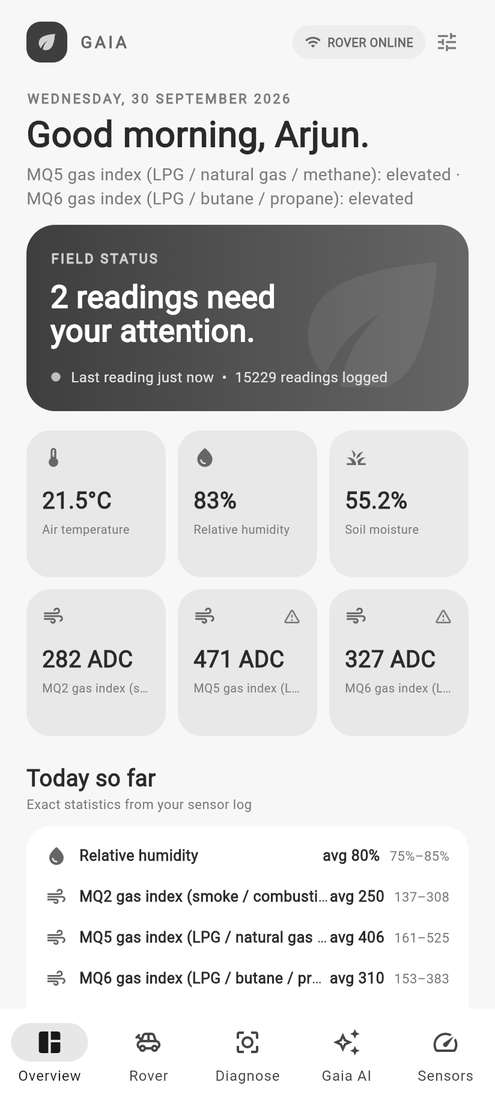
\includegraphics[height=95mm]{figures/app_overview.png}\\[2pt]\small (a) Overview\end{minipage}
\begin{minipage}{0.45\linewidth}\centering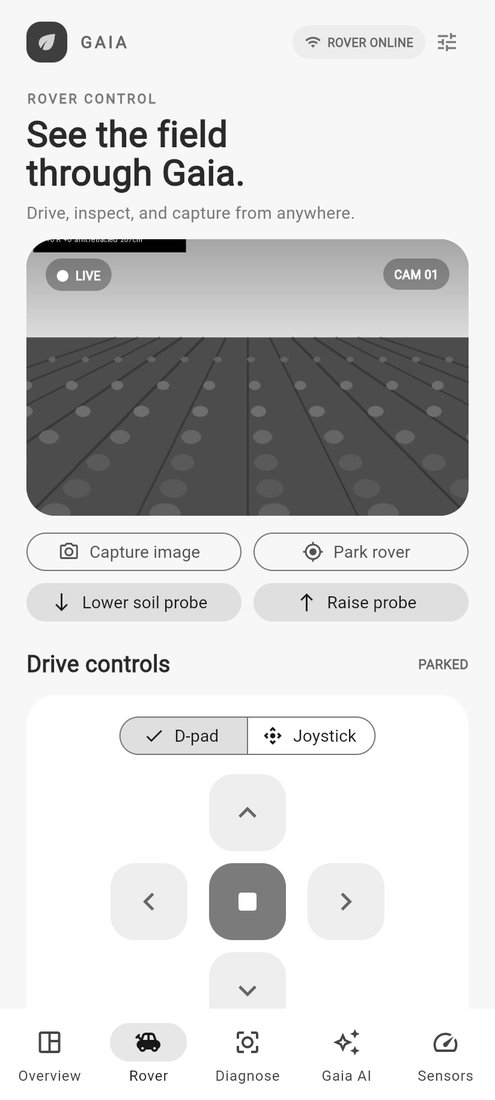
\includegraphics[height=95mm]{figures/app_rover.png}\\[2pt]\small (b) Rover control\end{minipage}
\caption{Mobile application: overview and rover control.}
\end{figure}

\begin{figure}[H]
\centering
\begin{minipage}{0.45\linewidth}\centering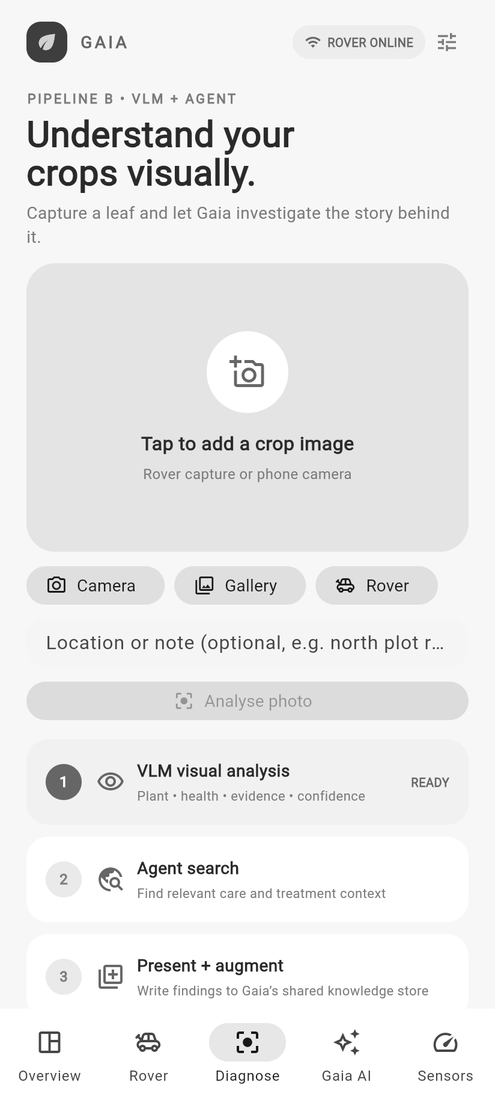
\includegraphics[height=95mm]{figures/app_diagnose.png}\\[2pt]\small (a) Diagnose\end{minipage}
\begin{minipage}{0.45\linewidth}\centering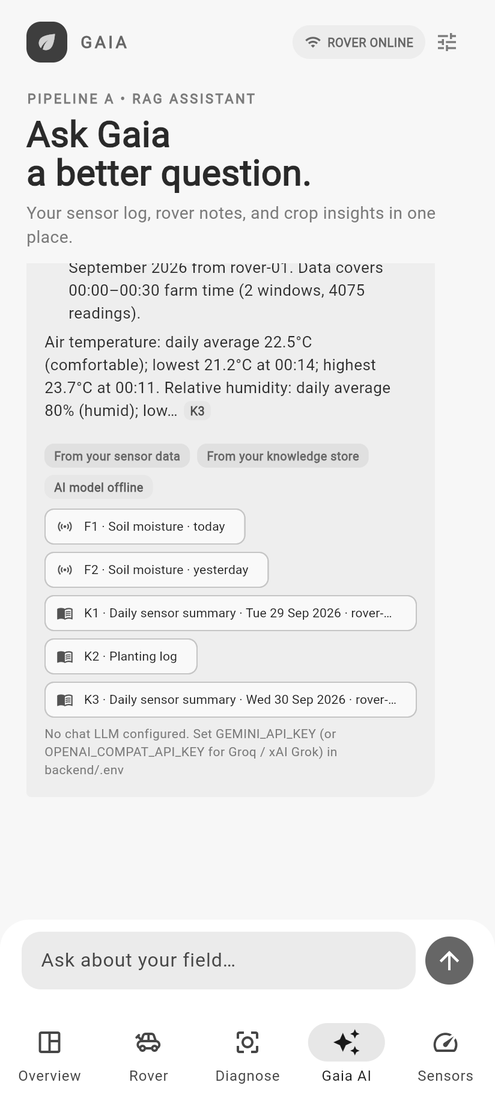
\includegraphics[height=95mm]{figures/app_chat.png}\\[2pt]\small (b) Gaia AI chat\end{minipage}
\caption{Mobile application: diagnosis and chat.}
\end{figure}

\begin{figure}[H]
\centering
\begin{minipage}{0.45\linewidth}\centering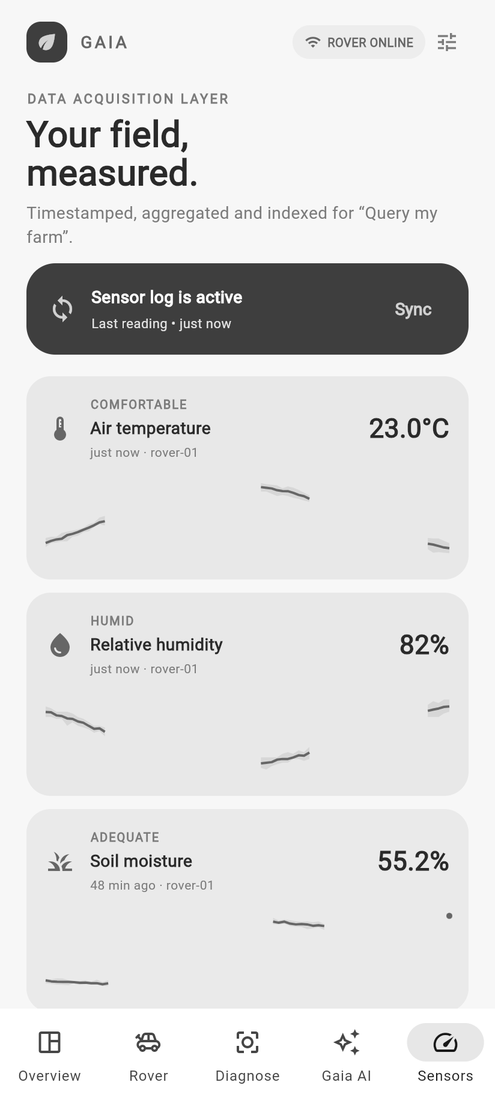
\includegraphics[height=95mm]{figures/app_sensors.png}\\[2pt]\small (a) Sensors\end{minipage}
\begin{minipage}{0.45\linewidth}\centering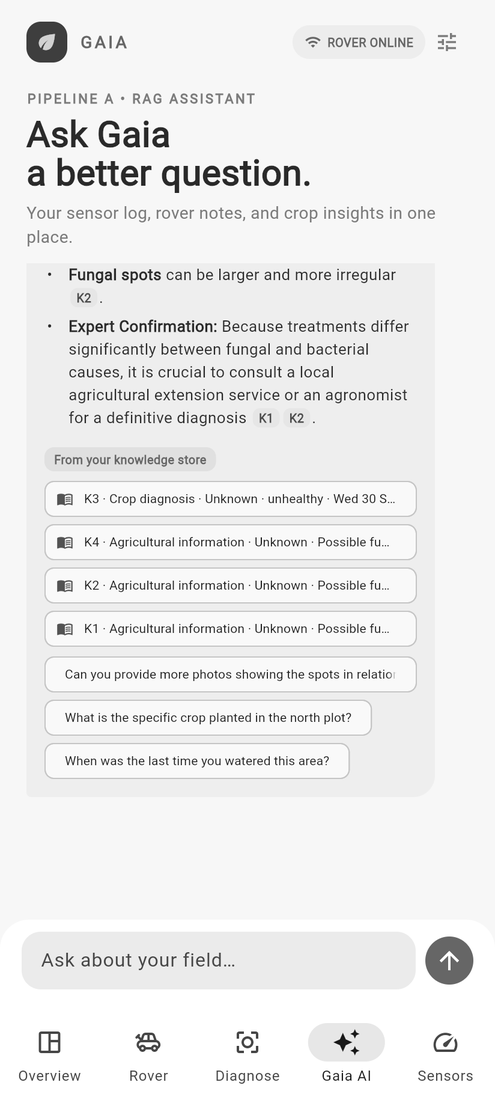
\includegraphics[height=95mm]{figures/app_chat_local_llm.png}\\[2pt]\small (b) Chat answer from a local model\end{minipage}
\caption{Mobile application: sensor values and a cited chat answer.}
\end{figure}

\begin{figure}[H]
\centering
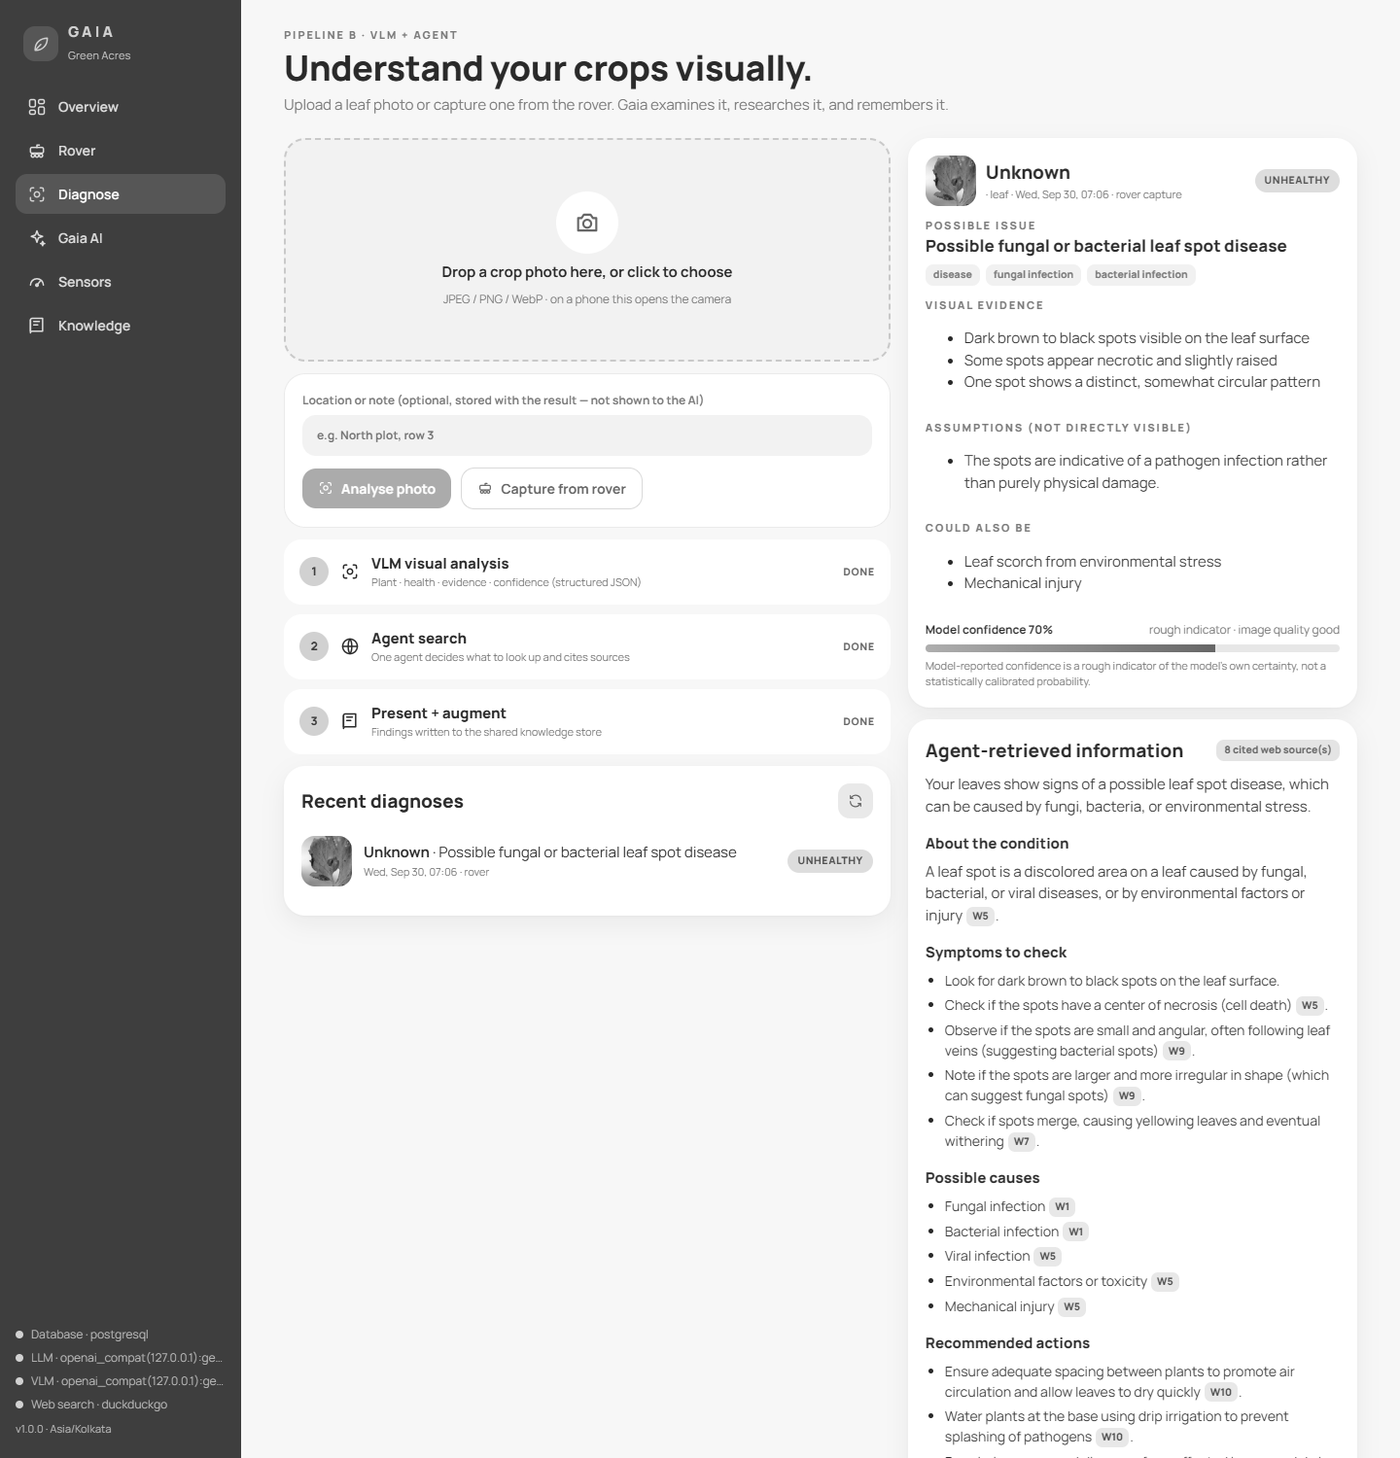
\includegraphics[width=0.88\linewidth]{figures/web_diagnosis_result_local_llm.png}
\caption{Web interface: a diagnosis result with evidence, confidence caveat and sources.}
\end{figure}

\begin{figure}[H]
\centering
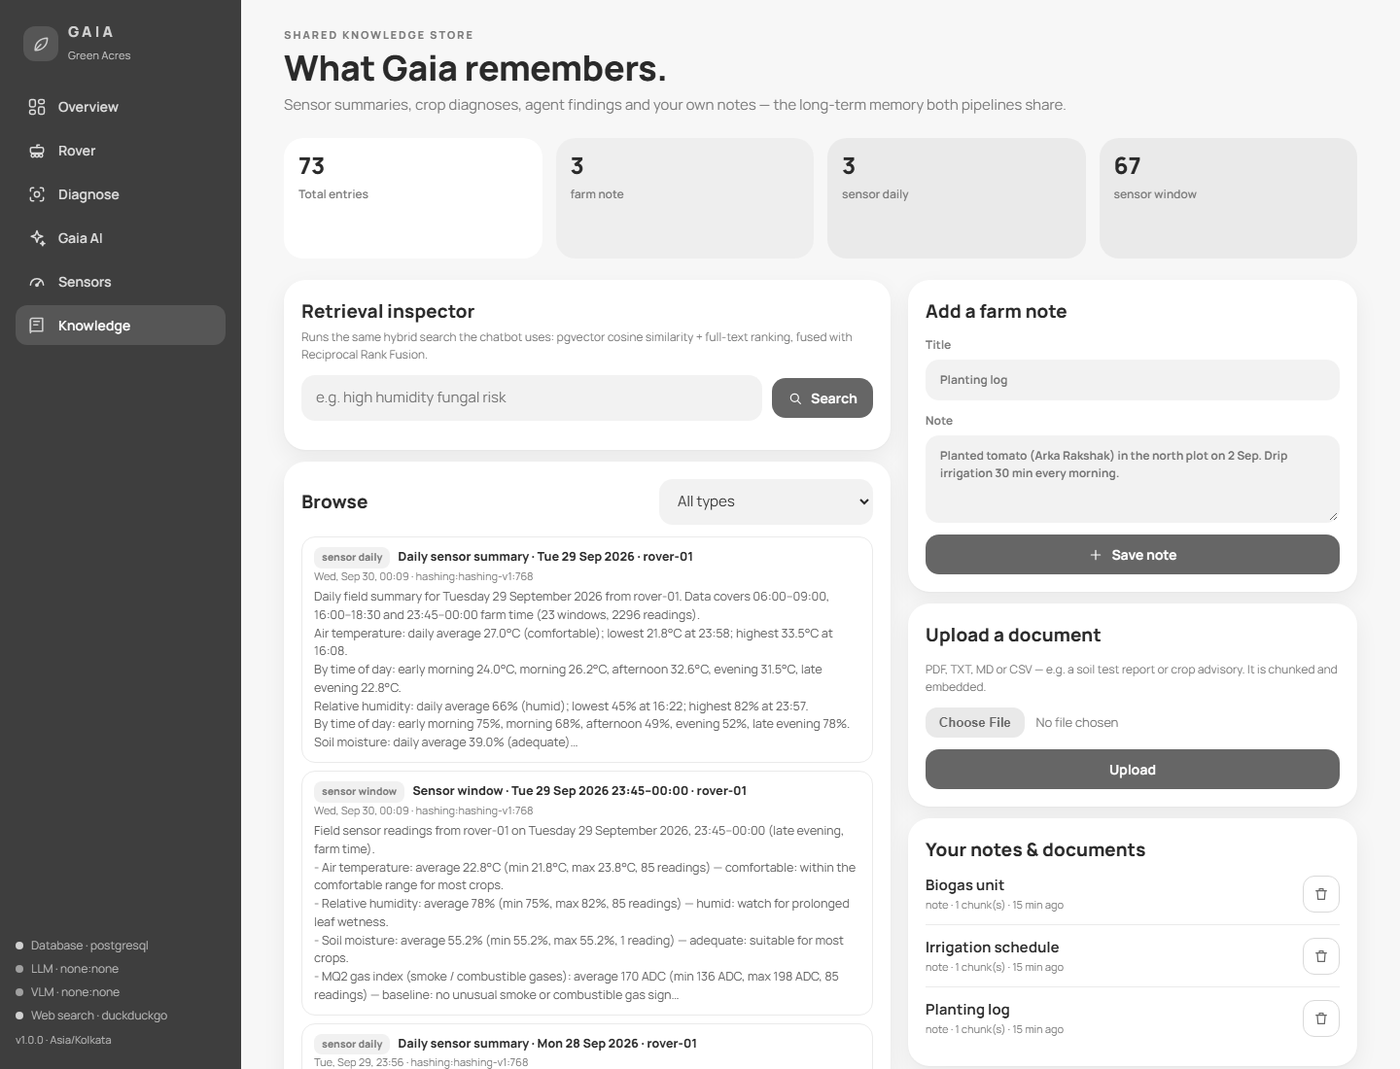
\includegraphics[width=0.88\linewidth]{figures/web_knowledge.png}
\caption{Web interface: knowledge-store inspector showing vector, lexical and fused scores.}
\end{figure}

\begin{figure}[H]
\centering
\imgslot[85mm]{app_live.png}{0.38}{Live view screenshot}\hspace{4mm}\imgslot[85mm]{app_switches.png}{0.38}{Rover tab with sensor switches}
\caption{Mobile application: Live view and per-sensor switches.}
\end{figure}

\begin{figure}[H]
\centering
\imgslot[85mm]{app_chat_stream.png}{0.38}{streamed chat answer}\hspace{4mm}\imgslot[85mm]{app_gap_answer.png}{0.38}{answer that explains a switched-off sensor}
\caption{Mobile application: streamed answer and gap explanation.}
\end{figure}

\begin{figure}[H]
\centering
\imgslot[70mm]{rover_front.jpg}{0.4}{rover, front or side view}\hspace{4mm}\imgslot[70mm]{rover_top.jpg}{0.4}{rover, top view with electronics}
\caption{The assembled rover.}
\end{figure}

\begin{figure}[H]
\centering
\imgslot[70mm]{rover_arm.jpg}{0.4}{soil-probe arm lowered}\hspace{4mm}\imgslot[70mm]{rover_field.jpg}{0.4}{rover in the field}
\caption{Soil-probe arm and field trial.}
\end{figure}
